\capitulo{Elementos de geometr\'ia diferencial}{Pedro Walter Lamberti}

\begin{epigrafe}
$\acute{\alpha} \gamma\epsilon \omega \mu \acute{\epsilon} \mu \acute{\epsilon} \tau \rho \eta \tau o \varsigma \;\; \mu \eta \delta
\epsilon \iota \varsigma \;\; \epsilon \iota \sigma \iota \tau \omega$  \\
Que no ingrese nadie que no sepa geometr\'ia.
\autortituloepigrafe{Frase grabada en la entrada de la Academia de Plat\'on}
\end{epigrafe}


% =============================== Estructuras =============================== %

\seccion{Estructuras}
\label{s:3.1}

Una  de  las  nociones m\'as  elementales  de  la  matem\'atica  es la  de  {\it
  Conjunto}.  Un   conjunto  es  una  colecci\'on   de  elementos  perfectamente
caracterizados.  Los   elementos  pueden  ser  de   cualquier  tipo:  n\'umeros,
funciones, personas, autos, etc. El  enfoque matem\'atico moderno es ir montando
estructuras de  distinta naturaleza sobre  un dado conjunto. En  este cap\'itulo
comenzaremos con la noci\'on de Espacio Topol\'ogico y llegaremos al concepto de
Variedad Riemanniana. Este procedimiento ha mostrado ser de utilidad en el marco
de la f\'isica, que es nuestro principal \'ambito de inter\'es.  El mapa de ruta
de  las de  las  distintas estructuras  que  veremos en  este  cap\'itulo es  el
siguiente:
%
\begin{itemize}
\item Espacio Topol\'ogico
\item Espacio M\'etrico
\item Variedad Topol\'ogica
\item Estructura Diferenciable (Variedad Diferenciable)
\item Estructura Afin (Noci\'on de paralelismo)
\item Estructura m\'etrica (Finsler y Riemann)
\end{itemize}

Si  bien   existe  una  estructura   intermedia  entre  la  topol\'ogica   y  la
diferenciable,  que se  conoce  como  {\it estructura  lineal  a trozos},  aquí
prescindiremos de su estudio. A  su vez, hay otras estructuras matem\'aticas que
son usadas en el marco de  las teor\'ias f\'isicas. Se destacan la estructura de
producto interno  sobre un conjunto complejo,  la cual conduce a  la noci\'on de
espacio  de Hilbert,  de fundamental  importancia en  Mec\'anica  Cu\'antica; la
estructura  simpl\'ectica, \'util  en Mec\'anica  Cl\'asica y  la  estructura de
Khaler, de relevancia en teor\'ia de cuerdas.

Comenzaremos con la noci\'on de espacio topol\'ogico.


%%%%%%%%%%%%%%%%%%%%%%%%%%%%%%%%%%%%%%

\subseccion{Espacio Topol\'ogico}

Un conjunto  arbitrario $X$  est\'a desprovisto de  toda estructura  que permita
definir nociones tales como la {\it convergencia} de una sucesi\'on de elementos
de  $X$, la  {\it proximidad}  de dos  elementos de  $X$, etc.  En  principio se
dispone s\'olo de las operaciones  elementales de {\it uni\'on} $\bigcup$ e {\it
  intersecci\'on} $\bigcap$ de  subconjuntos. Estas operaciones tambi\'en pueden
realizarse entre  distintos conjuntos.  Denotaremos con $\emptyset$  al conjunto
vac\'io.  Surge entonces el  desaf\'io entonces  de construir  alguna estructura
matem\'atica  definida sobre  $X$ que  permita  definir, de  manera precisa  las
nociones  de  proximidad,  continuidad,  convergencia,  etc.  Esto  se  logra  a
trave\'es de la idea de una {\bf topolog\'ia} sobre $X$.

\begin{definicion}
  Una  {\bf  Topolog\'ia}  $\tau$  sobre  el  conjunto $X$  es  una  familia  de
  subconjuntos de $X$ que cumple con las siguientes condiciones:
  %
  \begin{enumerate}
  \item $X$ y $\emptyset$ est\'an en $\tau$: $X, \emptyset \varepsilon \tau$ %
\item La intersecci\'on de cualquier colecci\'on finita de elementos de $\tau$ est\'a en $\tau$:
\[
A_i \varepsilon \tau, \forall i=1,...,n \Rightarrow \bigcap_{i=1}^n A_i \varepsilon \tau
\]
\item La uni\'on de una colecci\'on arbitraria - finita o no- de elementos de $\tau$, pertenece a $\tau$:
\[
A_{\alpha} \varepsilon \tau \Rightarrow \bigcup_{\alpha} A_{\alpha} \varepsilon \tau
\]
\end{enumerate}
\end{definicion}

\begin{definicion}
Al par $(X,\tau)$ lo llamaremos {\bf Espacio Topol\'ogico}. Los conjuntos que est\'an en $\tau$ se llaman {\it abiertos}.
\end{definicion}

{\it Ejemplos}:

\begin{itemize}
\item {\bf Topolog\'ia trivial}. Es la que consta de s\'olo dos elementos, el conjunto vac\'io y el conjunto total $X: \tau=\{\emptyset,X \}$
    
\item {\bf Topolog\'ia discreta}. Es la que en todo subconjunto de $X$ est\'a en $\tau$, es decir $\tau = \cal{P}(X)$ donde $\cal{P}(X)$ representa a las partes de $X$
    
\item En los cursos elementales de an\'alisis matem\'atico hemos estudiado en $\mathbb{R}^n$, es decir el conjunto de $n-tuplas$ de n\'umeros reales, la noci\'on de bolas abiertas. M\'as precisamente, una bola abierta en $\mathbb{R}^n$ centrada en el punto $p =(p_1,...,p_n) \varepsilon \mathbb{R}^n$ y de radio $r>0$ es el conjunto
    \[
{\cal{B}}_{r,p}={(x_1,...,x_n) \text{tal que   } 0\leq \sqrt{\sum_i (x_i-p_i)^2}<r}
\]
La colecci\'on de todas las bolas abiertas en $\mathbb{R}^n$ constituyen una topolog\'ia para $\mathbb{R}^n$. Se conoce como la {\bf topolog\'ia usual} de $\mathbb{R}^n$

\end{itemize}

\begin{definicion}
Un {\bf entorno} de un punto $x \varepsilon X$ es un conjunto $U$ que contiene a $x$ y tal que existe un abierto $V$ contenido en $U$: $x \varepsilon V \subseteq U$ con $U \varepsilon \tau$.
\end{definicion}

\begin{definicion}
Sea $f: X \rightarrow Y$ una funci\'on entre dos espacios topol\'ogicos $(X, \tau)$ e $(Y,\omega)$. $f$ es una {\bf funci\'on continua} en $x \varepsilon X$ sii dado cualquier entorno abierto $U \subset Y$ de $f(x)$, existe un entorno de $x$, $V \subset X$ tal que $f(V) \subset U$.
\end{definicion}

\begin{definicion}
Un {\bf homomorfismo} $\Psi$ entre dos espacios topol\'ogicos $(X,\tau)$ e $(Y,\omega)$ es una funci\'on
\[
\Psi: X \rightarrow V \subseteq Y
\]
biyectiva, continua y con inversa continua.
\end{definicion}

\begin{definicion}
Una {\bf sucesi\'on} en un conjunto $X$ es una aplicaci\'on $s: \mathbb{N} \rightarrow X$ donde $\mathbb{N}$ es el conjunto de los n\'umeros naturales. Denotaremos a la sucesi\'on por ${x_n} \text{donde  } n \varepsilon \mathbb{N}$
\end{definicion}

En un espacio topol\'ogico podemos introducir la noci\'on de convergencia de una sucesi\'on. Obs\'ervese que \'esto es posible gracias a que disponemos de la noci\'on de conjunto abierto.

\begin{definicion}
Sea $(X, \tau)$ un espacio topol\'ogico y $\{x_n\}, n \varepsilon \mathbb{N}$ una sucesi\'on en $X$. Diremos que $x$ es el {\bf l\'imite} de $x_n $ si para todo entorno $V$ de $x$, existe un $n_0 \varepsilon \mathbb{N}$ tal que $\forall n \geq n_0$ se tiene que $x_n \varepsilon V$.
\end{definicion}

Los l\'imites de las sucesiones no tienen porque ser \'unicos. Una condici\'on que debe cumplir el espacio topol\'ogico $(X,\tau)$ para que las sucesiones tengan un \'unico l\'imite es que dados dos puntos distintos $x \neq y$,con $ x,y \varepsilon X$ existen entornos disjuntos de $x$ e $y$.

A los espacios topol\'ogicos que satisfacen con esta condici\'on se los llama espacios de Hausdorff o espacio $T_2$.

\subseccion{Espacios m\'etricos}

En el tercer ejemplo de espacio topol\'ogico, usamos la noci\'on de m\'etrica eucl\'idea para definir las bolas abiertas en $\mathbb{R}$. El disponer de una m\'etrica no es algo que ocurre en todo conjunto. Eso motiva la siguiente definici\'on:

\begin{definicion}
Un {\bf Espacio M\'etrico} en un conjunto $X$ munido de una funci\'on $d: X \times X \rightarrow \mathbb{R}+$ tal que se cumplen las condiciones:
\begin{enumerate}
\item $d(x,y) \geq 0 \forall x,y \varepsilon X$ y la igualdad se cumple sii $x=y$
\item $d(x,y) = d(y,x)$
\item $d(x,y) \leq d(x,z)+d(z,y) \forall x,y,z \varepsilon X$
\end{enumerate}
\end{definicion}
La \'ultima condici\'on se conoce como {\it desigualdad triangular}. Mas adelante en este libro veremos funciones $d: X \times X \rightarrow \mathbb{R}^0$ que no satisfacen ni la condici\'on 2 ni la condici\'on 3, pero que sin embargo sirven para medir cu\'an separados est\'an dos puntos de $X$. En ese caso diremos que $d$ es una distancia en $X$.
\subseccion{Variedad Topol\'ogica}

Nuestra experiencia cotidiana de percibir que estamos inmersos en un espacio de 3 dimensiones, en el cual podemos medir \'angulos y determinar distancias entre dos puntos, ha hecho que usemos estas caracteristicas de nuestro habitat, como motivaci\'on de la defici\'on de ciertas estructuras matem\'aticas en espacios abstractos.

En primer lugar, con la noci\'on de una variedad topol\'ogica buscaremos simular en un conjunto cualquiera, la noci\'on de cercan\'ia y dimensionalidad que tenemos en $\mathbb{R}^n$.

\begin{definicion}
Una {\bf Variedad Topol\'ogica n-dimensional} es un espacio topol\'ogico $\mathcal{M}$ tal que es {\it localmente eucl\'ideo}, es decir que para cada $x \varepsilon {\cal{M}}$ existe un entorno abierto $U$ de $x$, homeomorfo a un abierto $V$ de $\mathbb{R}^n$:
\[
\phi: U \subseteq {\mathcal{M}} \rightarrow \mathbb{R}^n
\]
tal que
\[
\phi:U \rightarrow V
\]
y $\phi$ es un homeomorfismo. Tambi\'en pediremos que $\cal{M}$, como espacio topol\'ogico, sea un espacio Hausdorff.
\end{definicion}
A los pares $(U,\phi)$ se llaman cartas sobre $\mathcal{M}$. Se supone que la colecci\'on de todas las cartas cumbren completamente a $\mathcal{M}$. Las cartas permiten asignar {\it coordenadas} a $\mathcal{M}$:
\[
\text{Si  }p \varepsilon U \subseteq \mathcal{M} \text{   entonces  } \phi: p \rightarrow (p_1,...,p_n) \varepsilon\mathbb{R}^n  
\]
la colecci\'on de n\'umeros reales $(p_1,...,p_n)$ se llaman las coordenadas de $p$ de acuerdo a la carta $(U,\phi)$. Podr\'ia suceder que un mismo punto $p$ pertenezca a m\'as de una carta, digamos $(U_1,\phi_1)$ y $(U_2, \phi_2)$. En ese caso hablaremos de un cambio de coordenadas:
\begin{equation}\label{cc}
  \psi_2 \circ \phi_1^{-1}: \phi_(U_1 \cap U_2) \rightarrow \psi_2(U_1 \cap U_2)
\end{equation}
Si denotamos por $(p_1,...,p_n)$ a las coordenadas correspondientes a la carta $(U_1,\phi_1)$ y por $(\tilde{p}_1,...\tilde{p}_n)$ a las correspondientes a la carta $(U_2,\psi_2)$, entonces las funciones $\tilde{p}_i = \tilde{p}_i(p_1,...,p_n)$ son funciones continuas, y dan el cambio de coordenadas. Estas funciones son invertibles con inversa continua.

Ejemplos de variedades topol\'ogicas son:

$\circ \;\; \mathbb{R}^n$ En este caso hay una carta coordenada global que cubre toda la variedad y donde el homeomorfismo es la identidad.

$\circ \;\; S^n$, la esfera de dimensi\'on $n$. Est\'a definida como el conjunto:
\[
S^n = \{(x_1,...x_{n+1}), x_i \varepsilon \mathbb{R}, \text{  tales que   } x_1^2+...+x_{n+1}^2=1 \}
\]
Se debe observar que al definir $S^n$ no estamos pensando que est\'a inmersa en $\mathbb{R}^n$. 


%\begin{figure}[h!]
%\centerline{
\includegraphics[width=2cm]{logo_large}}
%
%\leyenda{Eso es  una figura, con  su leyenda sobre  varias lineas para  ver como
%  queda en el texto. Eso es una  figura, con su leyenda sobre varias lineas para
%  ver como queda en el texto.}
%\end{figure}


%\begin{table}
%\leyenda{Eso es un ejemplo de tabla}
%\begin{center}
%\begin{tabular}{|c|c|c|}
%\hline
%{\bf T\'itulo (negrita)} & {\bf T\'itulo (negrita)} & {\bf T\'itulo (negrita)}\\
%\hline
%A & Texto simulado (normal) & Texto simulado (normal)\\
%\hline
%B & Texto simulado (normal) & Texto simulado (normal)\\
%\hline
%\end{tabular}
%\fuente{Eso ser\'ia el fuente de la tabla}
%\end{center}\end{table}



\begin{figure}[h!]
\begin{center} 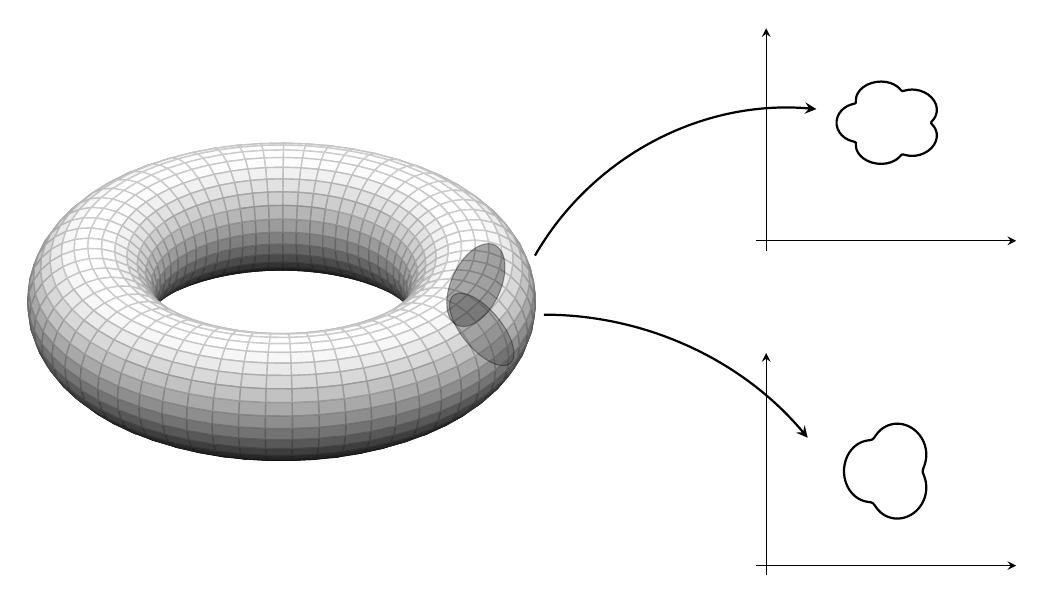
\begin{tikzpicture}[scale=1.25]
\shorthandoff{>}
\pgfplotsset{compat=1.6}
%
\pgfmathsetmacro\a{3} % rayon de rotation du centre du cercle definissant le tore
\pgfmathsetmacro\r{1} % rayon du cercle definissant le tore
%
\pgfmathsetmacro\au{.25} % 1/2 grand axe ellipse 1
\pgfmathsetmacro\bu{.45} % 1/2 petit axe ellipse 1
\pgfmathsetmacro\tu{25} % angle de rotation ellipse 1
%
\pgfmathsetmacro\ad{.2} % 1/2 grand axe ellipse 2
\pgfmathsetmacro\bd{.45} % 1/2 petit axe ellipse 2
\pgfmathsetmacro\td{-40} % angle de rotation ellipse 2
%
\pgfmathsetmacro\ru{.08} % rayon epitrocoide 1
\pgfmathsetmacro\ku{5} % ku-epicicotroide
\pgfmathsetmacro\du{.7} % \du*\ru = distance du point au centre (du = 1: epicicloide)
%
\pgfmathsetmacro\rd{.1} % rayon epitrocoide 2
\pgfmathsetmacro\kd{3} % ku-epicicotroide
\pgfmathsetmacro\dd{.6} % \du*\ru = distance du point au centre (du = 1: epicicloide) 
%
%
% Trace du domaine (tore)
% -----------------------------
%
\begin{axis}[axis equal image , clip=false , axis lines = none , colormap/blackwhite]
%y dir=reverse,
%axis on top
%
% Tore:
%view={45}{45}
\addplot3[domain = 0:360 , y domain = 0:360 , samples = 30 , samples y = 60 , surf , z buffer = sort]
({(\a+\r*cos(x))*sin(y)} , {(\a+\r*cos(x))*cos(y)} , {\r*sin(x)}); % ecuacion del tore
\end{axis}
%
% Ellipse 1
\filldraw[domain = 0:360 , samples=50 , fill = black , opacity = .35] plot 
({1.8*\a+\au*cos(\x)*cos(\tu)+\bu*sin(\x)*sin(\tu)} ,
  {.85*\a-\au*cos(\x)*sin(\tu)+\bu*sin(\x)*cos(\tu)});
%
% Ellipse 2
\filldraw[domain = 0:360 , samples=50 , fill = black!75 , opacity = .35] plot 
({1.82*\a+\ad*cos(\x)*cos(\td)+\bd*sin(\x)*sin(\td)} ,
  {.7*\a-\ad*cos(\x)*sin(\td)+\bd*sin(\x)*cos(\td)});
%
%
% Premier depliement
%
\draw[thick , domain = 0:360 , samples = 100 , yscale = .8] plot(
{3.2*\a+\ru*((\ku+1)*cos(\x)-\du*cos((\ku+1)*\x))} ,
{1.75*\a+\ru*((\ku+1)*sin(\x)-\du*sin((\ku+1)*\x))});
%
\draw[thick , >=stealth , ->]  ({2*\a},{.95*\a}) arc (150:85:3) ;
\draw[>=stealth , ->]  ({2.75*\a},{\a}) -- ({2.75*\a+5.5*\ru*(\ku+1)},{\a});
\draw[>=stealth , ->]  ({2.75*\a+.1},{\a-.1}) -- ({2.75*\a+.1},{\a+4.5*\ru*(\ku+1)});
%
%
% Second depliement
%
\draw[thick , domain = 0:360 , samples = 100 , yscale = 1.1] plot(
{3.2*\a+\rd*((\kd+1)*cos(\x)-\dd*cos((\kd+1)*\x))} ,
 {.2*\a+\rd*((\kd+1)*sin(\x)-\dd*sin((\kd+1)*\x))});
%
\draw[thick , >=stealth , ->]  ({2.03*\a},{.75*\a}) arc (90:40:3.5) ;
\draw[>=stealth , ->]  ({2.75*\a},{-.1*\a}) -- ({2.75*\a+5.5*\ru*(\ku+1)},{-.1*\a});
\draw[>=stealth , ->]  ({2.75*\a+.1},{-.1*\a-.1}) -- ({2.75*\a+.1},{-.1*\a+4.5*\ru*(\ku+1)});
\end{tikzpicture}
 \end{center}
\leyenda{Eso es la copia de la figura de Walter tomada en la red, que pas\'o en tikz}
\end{figure}